\documentclass{aastex62}   	% use "amsart" instead of "article" for AMSLaTeX format
\usepackage{graphicx}				% Use pdf, png, jpg, or eps§ with pdflatex; use eps in DVI mode
								% TeX will automatically convert eps --> pdf in pdflatex		
\usepackage{amssymb}
\usepackage{natbib}
\usepackage{grffile}

%SetFonts

%SetFonts

\begin{document}

\title{Testing Gravity using Type Ia Supernovae Discovered by LSST}
\author[0000-0001-6315-8743]{A.~G.~Kim}
\affiliation{    Physics Division, Lawrence Berkeley National Laboratory, 
    1 Cyclotron Road, Berkeley, CA, 94720}
\author{C.~Harper}
\affiliation{    Physics Division, Lawrence Berkeley National Laboratory, 
    1 Cyclotron Road, Berkeley, CA, 94720}
\author{C.~Ju}
\affiliation{    Physics Division, Lawrence Berkeley National Laboratory, 
    1 Cyclotron Road, Berkeley, CA, 94720}
\author{D.~Huterer}
\affiliation{Department of Physics, University of Michigan, 450 Church Street, Ann
Arbor, MI 48109, USA }

\author{others}

%\date{}							% Activate to display a given date or no date

\begin{abstract}
ZTF today and LSST in the upcoming decade will increase the number of identified  $z<0.3$ Type~Ia supernovae (SNe~Ia)  from the hundreds to the
hundreds of thousands.  The increase in the number density of SNe~Ia, in parallel with improvements in the standardization of
their absolute magnitudes, now make them competitive probes of the growth of structure.
\end{abstract}

\section{Connection between SNe~Ia and Gravity}


The growth of structure depends on the expansion history of the universe, the nature and density of its contents, and gravity. 
It is therefore a powerful probe of cosmology and dark energy.  Growth of structure can be measured from the baryonic structures
in the Universe and the peculiar velocities of test masses therein.
Peculiar velocities are motions, on top of the cosmological expansion, caused by the gravitational attraction
and repulsion of all sources of inhomogeneity in the Universe.

Baryonic structures and peculiar velocities  can provide a measurement of the combination $fD$, where $D$ is the linear growth factor that
gives the overall amplitude of  overdensities and
$$f \equiv \frac{d\ln{D}}{d\ln{a}}$$ is how that amplitude changes with redshift.  General Relativity predicts
$f=\Omega_M^\gamma$ (with $D$ determined accordingly) where $\gamma=0.55$, whereas other gravity models can be similarly described
but with different values of $\gamma$
\citep{2007APh....28..481L}.  Thus growth of structure, through the measurement of $fD$ (or $f\sigma_8$), provides a test of General Relativity.
We typically refer to $f\sigma_8$ because the  standard deviation of overdensities in 8$h^{-1}$Mpc spheres is often used to normalize the
overall amplitude of  overdensities.

As distance indicators SNe~Ia
can provide peculiar velocities (expressed equivalently as peculiar magnitudes)
of their host galaxies \citep{2006PhRvD..73l3526H,2011ApJ...741...67D}.  Existing SN~Ia samples
have been used to test and ultimately find spatial correlations in peculiar velocities, may be attributed to the growth of structure
\citet{2015JCAP...12..033H, 2017JCAP...05..015H}.  However, the signal-to-noise is currently insufficient to perform a meaningful test of GR.

Two advances in the upcoming decade will make SNe~Ia  important probes of $f\sigma_8$.
First, the precision of SN~Ia distances can be improved.  The commonly-used empirical 2-parameter SED model yields $\gtrsim 0.12$~mag distance modulus
dispersion.  However, SNe transmit more information than a light curve shape and single color used in current analysis.
Recent studies indicate that with the right data, SNe absolute
magnitudes can be calibrated to $\lesssim 0.08$ mag \citep[see e.g.][]{2012MNRAS.425.1007B, 2015ApJ...815...58F}.
As absolute magnitude uncertainty propagates into fractional velocity uncertainty, improvements to the standard candle lead to
improvements in their host peculiar velocities.
Secondly,  ZTF today and LSST in the upcoming decade will increase the number of identified  $z<0.3$ Type~Ia supernovae (SNe~Ia)  from the hundreds to the
hundreds of thousands.

The precision in  $f\sigma_8$ derived from an ten-year LSST-discovered  SN~Ia survey has been projected by \citet{2017ApJ...847..128H},
from both their  clustering and peculiar velocities.
The results are summarized in Table~\ref{tab:howlett}, where a 5\% distance uncertainty is assumed for each supernova.
SNe~Ia alone can provide a $2\%$ measurement of $f\sigma_8$ at $z<0.3$ redshifts lower than where galaxy, cluster, and Ly$\alpha$
RSD measurements are sensitive.

% Requires the booktabs if the memoir class is not being used
\begin{table}
   \centering
   %\topcaption{Table captions are better up top} % requires the topcapt package
   \begin{tabular}{@{} lccc @{}} % Column formatting, @{} suppresses leading/trailing space
	\hline
	Redshift & RSD & RSD + PV & cumulative\\ \hline
      $0.00<z<0.05$   & 66.3 & 13.9 & 13.9\\
     $0.05<z<0.10$            & 24.6     &  7.3 & 6.5\\
     $0.10<z<0.15$      & 14.8  & 5.8 & 4.3\\
     $0.15<z<0.20$      & 10.6  & 5.0 & 3.3\\
      $0.20<z<0.25$     & 8.3  & 4.4 & 2.6\\
     $0.25<z<0.30$  & 6.8  &  4.0 & 2.2\\
      \hline
   \end{tabular}
   \caption{Projected percent uncertainties in $f\sigma_8$ from a 10-year LSST SN survey with 5\% distance uncertainties from
   \citet{2017ApJ...847..128H}. RSD is from clustering, and RSD~+~PV is from joint clustering and peculiar velocities.
   The cumulative column shows the effective uncertainty from combining the redshift and all other shallower redshift bins.}
   \label{tab:howlett}
\end{table}

The projected precisions for LSST-discovered SNe~Ia have a number of interesting features.  Particular velocities contribute increasingly to
$f\sigma_8$ precision with decreasing redshift.  At redshift 0.3 the differential gain from adding peculiar velocities to the RSD measurement is small.
The differential gain in the cumulative $f\sigma_8$ constraint is small.  We therefore conclude that the focus should be in $z<0.3$ LSST SN~Ia discoveries.
After 10 years, the total number density of supernovae is such that both sample and shot noise contribute to the error budget for the volume with $z<0.2$, 
Galaxy RSD plus SN~Ia peculiar velocities have yet to be calculated.

They perform their analysis in Fourier space, 
where the Fisher information matrix of a random Gaussian field with mean zero and covariance $C(k)$ parameterized by $\lambda$ is
approximated by
\begin{equation}
F_{ij} = \frac{V}{2}\int \frac{d^3k}{(2\pi)^3} \text{Tr}\left[ C^{-1} \frac{\partial C}{\partial \lambda_i} C^{-1}
\frac{\partial C}{\partial \lambda_j} \right],
\end{equation}
where the he covariance
\begin{equation}
C = P_{vv}(k) + \frac{\sigma^2}{n}
\end{equation}
has contributions from the power spectrum, noise in the velocity measurement, and the density of velocity probes
\citep{2017MNRAS.464.2517H}. 
In the sample variance limit for a sample with fixed depth, the variance in $f\sigma_8$ (and other $\lambda$ parameters)
is thus inversely proportional to the survey solid-angle $\Omega$, whereas
in the shot-noise limit the variance is inversely proportional to $\Omega n^2 \propto N^2/\Omega$, where $n$ is the number density,
and $N$ is the total number of supernovae.  

While there have been a number of articles on the subject,
our analysis brings a higher level of fidelity than sought by previous analyses.  We simulate SNe~Ia hosted by galaxies in a mock galaxy
catalog. The numbers of SNe are sufficiently small to allow fast evaluations of the likelihood, which enable the determination of parameter
posteriors using MCMC on reasonable computing timescales.   We can use our machinery to 
compare different survey parameters, such as redshift depth, total numbers of supernovae,
solid angle/survey geometry, and SN~Ia intrinsic magnitude dispersion.

The motivation of this work is to quantify the probative power of SN~Ia-derived peculiar velocities in the LSST era.


We consider a maximum redshift of $z=0.2$ because over ten years the noise is not shot-noise dominated, meaning that the differential improvement
in the precision of
$f\sigma_8$ due to a lower-redshift supernova is greater than that due to a high-redshift supernova.  Following all LSST SNe~Ia below this redshift 
likely saturate available follow-up resources.
Our calculations are thus based on the number and solid-angle of $z<0.2$ supernova pre-maximum discoveries 
for the survey candidates provided by the Project.  Based on these numbers we calculate the Figures of Merit in
both sample and shot-noise limits, normalized to ``baseline2018a''.
After 10 years,
LSST supernovae are at neither extreme; we thus adopt the average of the two FoM's as what we advocate for the survey.
These averages for a select set of surveys are shown in Figure~\ref{fig:fom}.

The cross-correlation between galaxy-count and peculiar-velocity surveys is not yet implemented but is a planned extension of this work.  We would like to
quantify the suppression of sample variance achieved when considering matter-densities and velocities 
within the same volume \citep{2007PhRvL..99h1301G}.

\section{Simulated Data}
The Buzzard (v1.6) galaxy catalog is used.  This is because it is the survey, with a light cone that covers 10,313.24 sq.~deg., that covers
the largest solid angle among those currently available
in the DESC Generic Catalog Reader.  However,
the survey geometry is different
from that of LSST.  The catalog is based on a Flat $\Lambda$CDM model with $H_0=70$~km~s$^{-1}$,  $\Omega_M=0.286$, $\Omega_B=0.047$, and
$\Omega_\nu=0$.
The catalog contains 140M galaxies with observed redshift $z<0.2$.
Each galaxy has its cosmological redshift, the $x$-, $y$-, $z$-components of its peculiar velocity from which
the radial peculiar velocity is determined, and its
star formation rate and stellar mass from which the
supernova rate of each host is determined using 
\citet{2012ApJ...755...61S}.  Supernovae are realized for a span of 10 observer-years yielding 17,205 objects.  This total supernova
production underestimates the expected discovery of 130,000 supernovae in 10 observer-years based on the volumetric
rate of \citet{2010ApJ...713.1026D}.  The volumetric rate is more robust, so the sample under consideration in this article
corresponds to 1.3 years worth of discoveries. 

Each supernova is assigned a magnitude based on the distance modulus of its cosmological
redshift plus a random term drawn from a Normal distribution $\sigma_M$, which for simplicity is the same for all supernovae and captures both
intrinsic magnitude dispersion and measurement uncertainty.  No other corrections are applied to the observed magnitude.  Dipole effects of the heliocentric
motion with respect to the CMB and of the galaxies with respect to the CMB  are ignored: referring to
\citet{2011ApJ...741...67D}, the effects in Eq.~18 are ignored.

\section{Analysis}
The analysis of this article is  almost identical to that of \citet{2015JCAP...12..033H, 2017JCAP...05..015H}.   The peculiar magnitude correlation
function $\xi_{\delta m \delta m}$ expected from General Relativity starting with the CMB
matter density power spectrum is calculated using CAMB \citep{Lewis:2002ah}  assuming the same
cosmological parameters used for the Buzzard catalog.  Our model for the data covariance
is
\begin{equation}
C_{ij} = A\xi_{\delta m \delta m}(\mathbf{r_i},\mathbf{r_j}) + \frac{\sigma_M^2}{N_i} \delta_{ij} + \sigma^2_{NL}(z_i;\sigma_{v})\delta_{ij}.
\end{equation}
In this model, we treat the shape of the power spectrum $\xi$ as fixed and use the parameter $A$ to represent
deviations from General Relativity $A=1$.  This model is not sensitive to  the shape of
the power spectrum between gravitational models.  Nevertheless, for
convenience we say that our model gives $f\sigma_8 = A (f\sigma_8)^{GR}$, where $(f\sigma_8)^{GR}$ is the expectation
from General Relativity.  Special cases of modified gravity could give $A=1$, but inconsistency with $A=1$ is is evidence against General Relativity.
The final term includes extra magnitude dispersion produced by non-linear effects on velocity, parameterized with $\sigma_{v}$, such that
\begin{equation}
\sigma_{NL} = \frac{5}{\ln{10}} \frac{1+\bar{z}}{\bar{z}} \sigma_v,
\end{equation}
where $\bar{z}$ is the cosmological redshift of the host galaxy.
\section{Results of Subsets}

For all analyses we remove supernovae below observed $z_{min}=0.01$ in order to
reduce errors made in the first-order transformation between velocity and
magnitude.  This cut removes a  small volume relative to the full survey.

The 
\begin{figure}
\centering
\includegraphics[width=0.5\textwidth]{../outcosmo/pvlist.0.08.1234.1.0.2.pkl.png}
\caption{Confidence regions for the model parameters.  $A=(f\sigma_8)/(f\sigma_8)_{GR}$, $M$ is the supernova
absolute magnitude, $\sigma_M$ is the magnitude dispersion, and $\sigma_v$ is the non-linear contribution
to peculiar velocity.   The parameters for which I controlled the input, $M=0$ and $\sigma_M=0.08$~mag, are shown in dotted lines.
 Left: A survey truncated at $z_{max}=0.1$.  Right: A survey truncated at $z_{max}=0.15$.
\label{zmax:fig}}
\end{figure}


\begin{table}
   \centering
   %\topcaption{Table captions are better up top} % requires the topcapt package
   \begin{tabular}{|cccc|cccc|} % Column formatting, @{} suppresses leading/trailing space
   \hline
$z_{max}$ & fraction & $\sigma_{SN}$ & $N_{gal}$ & $\bar{A}$ & $\sigma_A$ & $\sigma_A N_{gal}^{-0.5}$ & $\bar{A} \sigma_A^{-1} (18000/760)^{0.5}$ \\
\hline
0.20 &  1.0 & 0.08 & 9901 &   1.18 &   0.23 &  0.050 &  24.38 \\ \hline
0.20 &  0.2 & 0.08 & 2021 &   1.66 &   0.59 &  0.062 &  13.61 \\
0.20 &  0.3 & 0.08 & 3023 &   1.34 &   0.43 &  0.057 &  15.16 \\
0.20 &  0.5 & 0.08 & 5015 &   1.13 &   0.30 &  0.054 &  18.54 \\
0.10 &  1.0 & 0.08 & 1294 &   0.91 &   0.28 &  0.091 &  15.96 \\
0.15 &  1.0 & 0.08 & 3870 &   1.00 &   0.24 &  0.066 &  20.00 \\
0.20 &  1.0 & 0.10 & 9901 &   1.06 &   0.25 &  0.042 &  20.33 \\
0.20 &  1.0 & 0.12 & 9901 &   1.09 &   0.28 &  0.040 &  19.13 \\
0.15 &  0.3 & 0.12 & 1215 &   1.97 &   0.92 &  0.061 &  10.36 \\
0.12 &  0.3 & 0.10 & 746 &   1.62 &   0.70 &  0.085 &  11.28 \\
0.07 &  1.0 & 0.08 & 563 &   1.16 &   0.36 &  0.135 &  15.55 \\
    \hline
   \end{tabular}
   \caption{.}
   \label{tab:booktabs}
\end{table}


We consider two different scenarios cutting at different redshift depths $z_{max}=0.1$ and  $z_{max}=0.15$.  All the objects in the first
scenario are in the second scenario.  The results are shown in Fig.~\ref{zmax:fig}.  The points of interest are:
\begin{itemize}
\item There is a bias toward low $f\sigma_8$ for low-redshift ($z_{max}=0.1$).  Adding more supernova with increasing redshift
 decreases the bias  ($z_{max}=0.15$), and $A$ eventually approaches 1 ($z_{max}=0.2$ not shown).
 \item Based on the analysis of \citet{2017MNRAS.471.3135H}, I added an intrinsic velocity dispersion $\sigma_v$ (km~s$^{-1}$) due to non-linear effects.  This was not
 in Dragan's model.  My fit finds that this  dispersion is consistent with zero, not well constrained, and not strongly correlated with
 $A$.  The lack of covariance is consistent with Dragan's own tests.
 \item The fit intrinsic magnitude dispersion, on the other hand, is larger than the input $\sigma_M=0.08$ mag.  This  indicates that the catalogs
 contain 
 extra  velocity dispersion better attributed to intrinsic magnitude dispersion rather than correlated peculiar velocities.
\end{itemize}


\begin{figure}
\includegraphics[width=0.5\textwidth]{../outcosmo/pvlist.0.08.1234.1.0.1.pkl.png}
\includegraphics[width=0.5\textwidth]{../outcosmo/pvlist.0.08.1234.1.0.2.pkl.png}
\caption{Confidence regions for the model parameters.  $A=(f\sigma_8)/(f\sigma_8)_{GR}$, $M$ is the supernova
absolute magnitude, $\sigma_M$ is the magnitude dispersion, and $\sigma_v$ is the non-linear contribution
to peculiar velocity.   The parameters for which I controlled the input, $M=0$ and $\sigma_M=0.08$~mag, are shown in dotted lines.
 Left: A survey truncated at $z_{max}=0.1$.  Right: A survey truncated at $z_{max}=0.2$.
\label{zmax:fig}}
\end{figure}

\begin{figure}
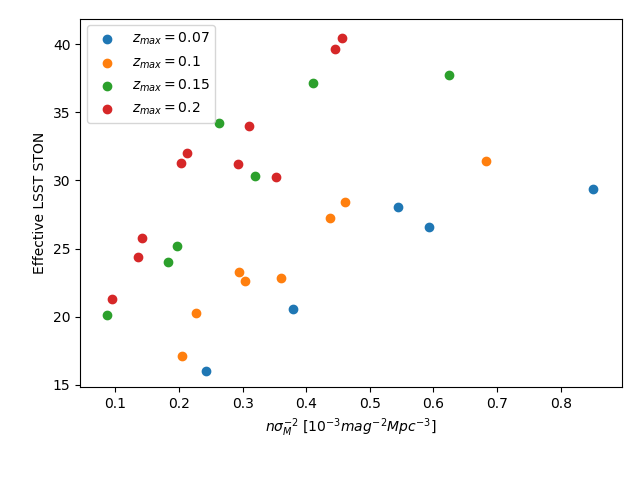
\includegraphics[width=0.5\textwidth]{../outcosmo/fracsnsig2_.png}
\includegraphics[width=0.5\textwidth]{../outcosmo/zmax_.png}
\caption{Confidence regions for the model parameters.  $A=(f\sigma_8)/(f\sigma_8)_{GR}$, $M$ is the supernova
absolute magnitude, $\sigma_M$ is the magnitude dispersion, and $\sigma_v$ is the non-linear contribution
to peculiar velocity.   The parameters for which I controlled the input, $M=0$ and $\sigma_M=0.08$~mag, are shown in dotted lines.
 Left: A survey truncated at $z_{max}=0.1$.  Right: A survey truncated at $z_{max}=0.15$.
\label{zmax:fig}}
\end{figure}

\begin{itemize}
\item Dragan: Is there some way that the formalism in your article breaks down at low-redshift?  I do remove very low-redshift objects at $z<0.01$,
which I think is conservative.
 \item Risa/Joe: Is there any reasons for the Buzzard catalog to not capture correlated peculiar velocities on small scales (box size to large?) nor capture
 non-linear velocities?  (I don't know how to translate a mass resolution of 2.7e10 $M_{\odot}/h$ into a spatial resolution!)
\end{itemize}

\bibliographystyle{aasjournal}
\bibliography{/Users/akim/Documents/alex}

\end{document}  